
\section{Result}
In this section, we show the results of our experiments obtained. To evaluate the performance of our proposed self-supervised InfNet, we compare its performance with other state-of-the-art methods including the original InfNet.

\subsection{Result comparison for Single InfNet}
Table \ref{tab:single} shows the result for the single segmentation InfNet. The single segmentation InfNet does not segment between ground-glass opacities or consolidation. The single segmentation segments and represents all infected region as one. We can see that self-supervision can improve on the generalization and consistency in predicting the different CT lung images as they perform the best in terms of the error range. Even though the baseline single InfNet (Single SInfNet) performance has better mean values for F1, IoU, and Recall, the self-supervised approach helps to create robustness and consistency in the model itself to better handle outliers. We can see the results of the single segmentation in Figure \ref{fig:single-comparison}. We can see that the baseline single InfNet (Single SInfNet) overestimated the infected region of an outlier in the segmentation result in the figure in the last row. The self-supervised Single InfNet (Single SSInfNet) did a better job at predicting outliers where its prediction is more closely related to the ground truth than the baseline single SInfNet (Single SInfNet). The receiving operating characteristics (ROC) can be seen in Figure \ref{fig:single_rocs}. The baseline Single InfNet (Single SInfNet) has the best performing ROC.
 
  \begin{figure*}
 	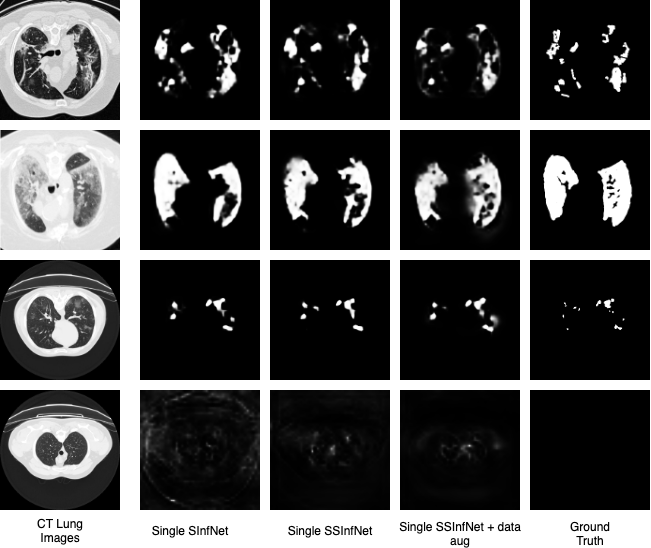
\includegraphics[width=\linewidth]{comparison_single.png}
 	\caption{Comparison of single segmentation between different networks. Overall, the Single SInfNet achieves a better performance than the rest of the network as seen in row 1 to row 3. However, our method by adding self-supervised to InfNet (Single SSInfNet) prevents overestimating the infected region of the CT lung images as can be seen in row 4.}
 	\label{fig:single-comparison}
 \end{figure*}

 \begin{figure*}
 	\centering
 	\small
 	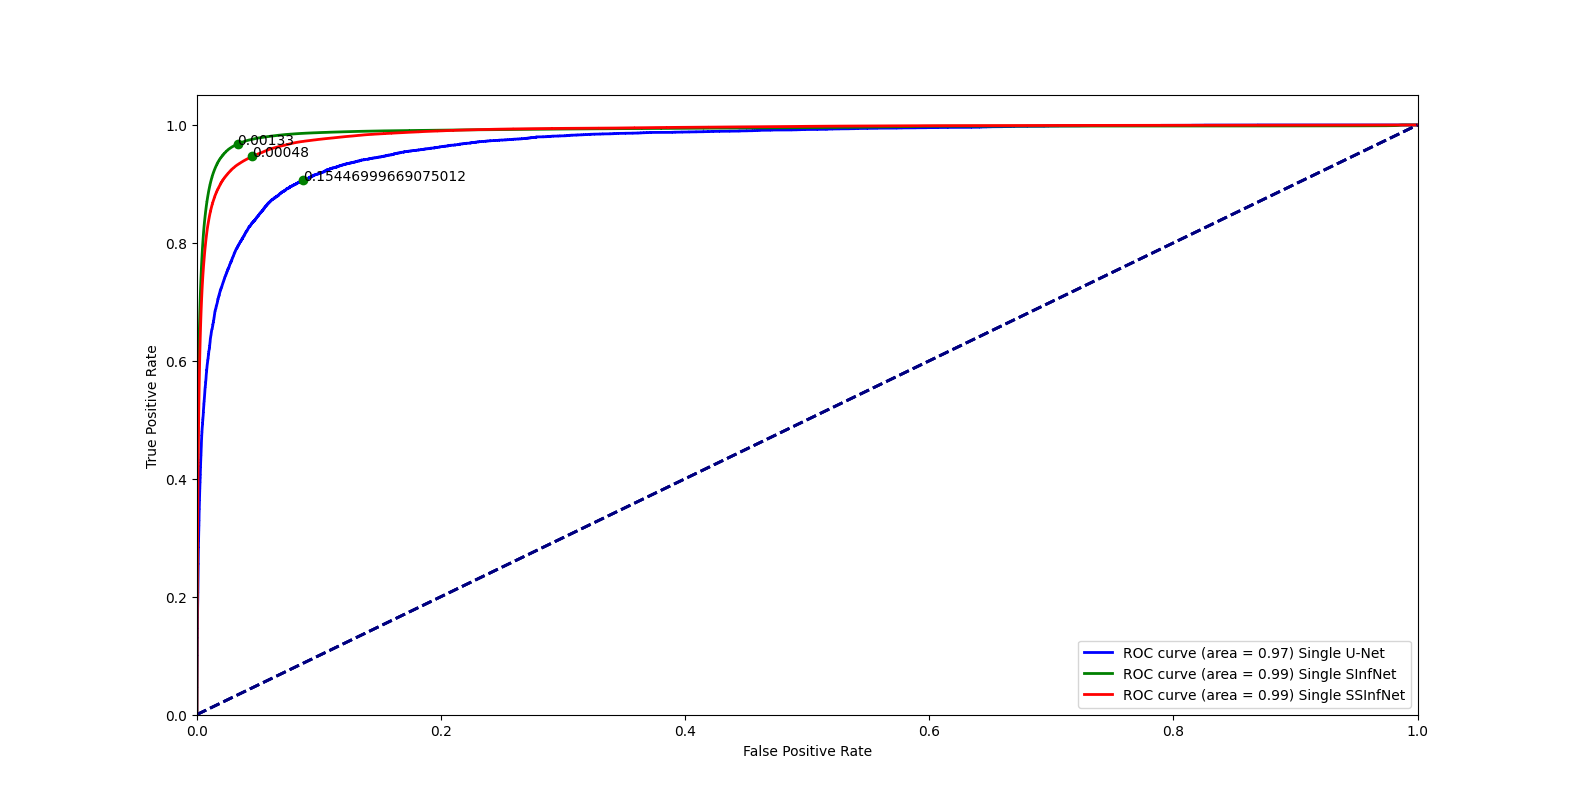
\includegraphics[width=\linewidth]{single_rocs.png}
 	\caption{ROC comparison of different networks.}
 	\label{fig:single_rocs}
 \end{figure*}
 
 \begin{table*}[!ht]
 	\centering
 	\begin{tabular}{| c | c || c c c c c ||}
 		\hline
 		Methods & & F1 & IoU & Recall & Precision & AUC \\ \hline
 		Single U-Net & Mean & 0.13 & 0.08 & 0.60 & 0.08 & 0.8818 \\ \cline{2-7}
 		& Error & $\pm$0.033 & $\pm$0.023 & $\pm$0.090 & $\pm$0.025 & $\pm$0.027 \\ \hline
 		Single SInfNet &  Mean & \textbf{0.43} & \textbf{0.32} & \textbf{0.82} & \textbf{0.38} &0.9604 \\ \cline{2-7}
 		& Error & $\pm$ 0.060 & $\pm$ 0.055 & $\pm$0.069 & $\pm$0.058  & $\pm$0.032 \\ \hline
 		Single SSInfNet &  Mean & 0.38 & 0.27 & 0.75 & 0.33 & \textbf{0.9742}  \\ \cline{2-7}
 		& Error & $\pm$0.056 & $\pm$0.049 &$\pm$0.077  & $\pm$0.053 & $\pm$  0.010 \\ \hline
 	\end{tabular}
 	\caption{Quantitative result for comparison between Single segmentation InfNet and self-supervised single segmentation InfNet in the test set. Single SSInfNet is our self-supervised single InfNet.}
 	\label{tab:single}
 \end{table*}


\subsection{Results comparison for Multi InfNet}
Table \ref{tab:multi-weakprior} shows the result for the comparison between multiple segmentation InfNet. As the multiple segmentation InfNet requires a CT lung image concatenate with a prior as input where the prior is the segmentation of the infected region of the CT lung without considering the location of ground-glass opacities or consolidation. The prior represents the infected region as a whole. The prior is obtained by running prediction of the infected region by the single segmentation InfNet on the CT lung images of the test set. Then the prior is fed together with the CT lung image from the test set into the multiple segmentation InfNet to obtain the result. As the baseline Single InfNet (Single SInfNet) achieves the best performing single InfNet, we use the prediction of the prior obtained from the baseline Single InfNet to be fed into the multi segmentation InfNet with the CT lung images. The self-supervised Multi InfNet (SSInfNet) was able to achieve a higher performance than the baseline Multi InfNet (SInfNet). The self-supervised Multi InfNet (SSInfNet) achieves the best performance in evaluating the ground-glass opacities and the consolidation area of the CT lung images than the baseline Multi InfNet (SInfNet). The overall performance of the self-supervised Multi InfNet (SSInfNet) achieves the best result. We can see the segmentation result in Figure \ref{fig:multi-weakprior-comparison}. However, the baseline Multi InfNet (SInfNet) achieves a better recall score than the rest of the networks. As we can see in Figure \ref{fig:multi-weakprior-comparison}, the baseline multi InfNet (SInfNet) predicted more of the consolidation even on areas that is not infected. On the third row, the SInfNetoverestimated the consolidation area in the healthy CT lung image. As recall is the amount of true positive over the total actual consolidation area, the SInfNet seems to overestimated the consolidation area which results in a higher recall score than the other networks. However, as most of the prediction of the consolidation area for the SInfNet is not accurate, the precision for the SInfNet is lower. This therefore decreases the performance of the SInfNet.


\begin{table*}[!h]
	\centering
	\begin{tabular}{ |c|c|c|c|c|c|c|c| }
		\hline
		Methods & & \multicolumn{2}{c|}{U-Net} & \multicolumn{2}{c|}{SInfNet} & \multicolumn{2}{c|}{SSInfNet}  \\ \hline
		&  &mean & error & mean & error & mean & error \\ \hline
		
		\multirow{4}{*}{\rotatebox[origin=c]{90}{GGO}} 
		& F1 & 0.26 & $\pm$0.057 & 0.38 &$\pm$0.054 & \textbf{0.43} & $\pm$0.057 \\ \cline{2-8}
		& IoU & 0.18 &$\pm$0.043 &0.27 &$\pm$0.042 &
		\textbf{0.31} &$\pm$0.046 \\ \cline{2-8}
		& Recall & 0.216 &$\pm$0.053 &\textbf{0.58} &$\pm$0.065 &\textbf{0.58} &$\pm$0.072 \\ \cline{2-8}
		& Precision & 0.405 &$\pm$0.085 &0.41 &$\pm$0.058 &
		\textbf{0.48}\^ &$\pm$0.059 \\ \cline{2-8}
		\hline \hline
		
		\multirow{4}{*}{\rotatebox[origin=c]{90}{Cons}} 
		& F1 & 0.35 &$\pm$0.097 &0.29 &$\pm$0.078 &\textbf{0.46}*\^ &$\pm$0.096 \\ \cline{2-8}
		& IoU & 0.26& $\pm$0.08&0.22 &$\pm$0.068 &\textbf{0.36}*\^ &$\pm$0.088 \\ \cline{2-8}
		& Recall &0.32 &$\pm$0.089 &\textbf{0.61} &$\pm$0.099 &0.56 &$\pm$0.11 \\ \cline{2-8}
		& Precision & 0.46 &$\pm$0.116 &0.31 &$\pm$0.084 &\textbf{0.56}*\^ &$\pm$0.101 \\ \cline{2-8}
		\hline \hline
		
		\multirow{4}{*}{\rotatebox[origin=c]{90}{Background}} 
		& F1 & 0.857&$\pm$0.01 &1.0 &$\pm$0.002 &1.0 &$\pm$0.002 \\ \cline{2-8}
		& IoU & 0.754&$\pm$0.017 &0.99 &$\pm$0.003 &0.99 &$\pm$0.003 \\ \cline{2-8}
		& Recall &0.998 &$\pm$0.001 &0.99 &$\pm$0.002 &0.99 &$\pm$0.002 \\ \cline{2-8}
		& Precision &0.755 &$\pm$0.017 &1.0 &$\pm$0.002 &1.0 &$\pm$0.002 \\ \cline{2-8}
		\hline \hline
		
		\multirow{4}{*}{\rotatebox[origin=c]{90}{Overall}} 
		& F1 &0.49 &$\pm$0.055 &0.55 &$\pm$0.044 &\textbf{0.63}* &$\pm$0.052 \\ \cline{2-8}
		& IoU & 0.40 &$\pm$0.046 &0.5 &$\pm$0.038 &\textbf{0.55} &$\pm$0.046 \\ \cline{2-8}
		& Recall &0.51 &$\pm$0.048 &\textbf{0.73} &$\pm$0.055 &0.71 &$\pm$0.061 \\ \cline{2-8}
		& Precision &0.54 &$\pm$0.073 &0.57 &$\pm$0.048 &\text
		bf{0.68}* &$\pm$0.054 \\ \cline{2-8}
		\hline \hline
		
	\end{tabular}
\caption{Quantitative result of Ground-glass Opacities \& Consolidation on the test data set. Prior is obtained from the single segmentation InfNet. SSInfNet is our self-supervised multi InfNet. GGO: Ground-Glass Opacity. Cons: Consolidation. A p-value is calculated using t-test to compare the performance between the SSInfNet and the SInfNet. For values where the p-value is less than 0.05 and is significant as calculated with the t-test, they are marked with *. For values calculated with Wilcox test and have p-value of less than 0.05, they are marked with \^. }
\label{tab:multi-weakprior}
\end{table*}


  \begin{figure*}
 	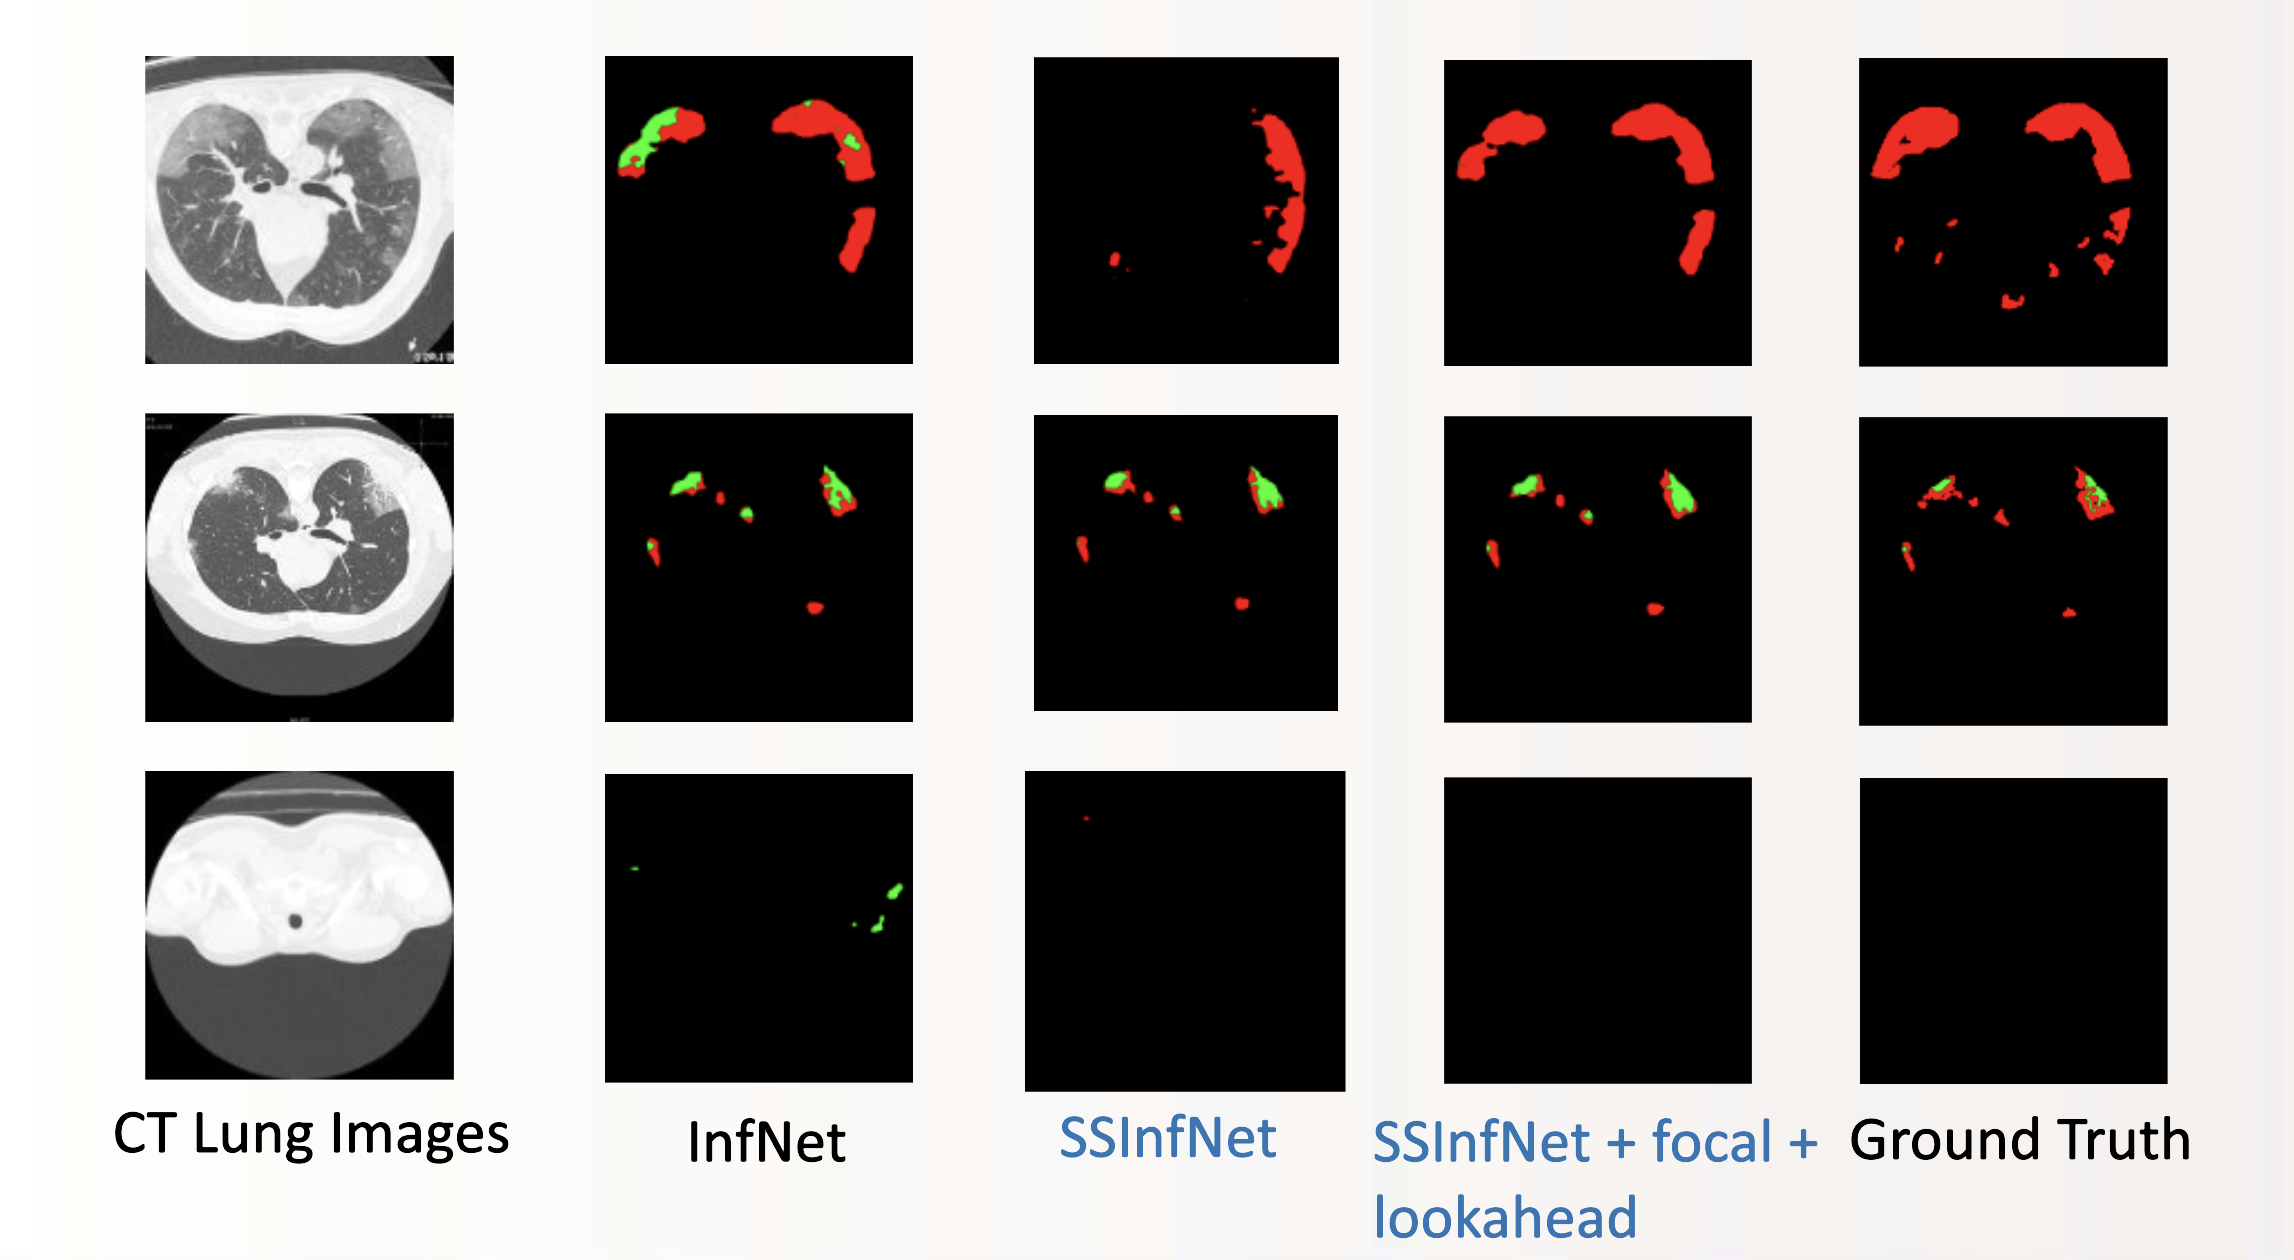
\includegraphics[width=\linewidth]{comparison_multi_weakprior.png}
 	\caption{Comparison of multi segmentation between different networks with prior generated from single InfNet. Red colored is the ground-glass opacities and green colored is the consolidation. The baseline multi InfNet (SInfNet) overestimated the consolidation region in the first and third row of the CT lung image when there are not suppose to be any consolidation region.}
 	\label{fig:multi-weakprior-comparison}
 \end{figure*}
